\documentclass[journal,a4paper]{IEEEtran}

% ─── Core Packages ────────────────────────────────────────────────────────────
\usepackage[T1]{fontenc}
\usepackage[utf8]{inputenc}
\usepackage{amsmath,amssymb,amsfonts}
\usepackage{graphicx}
\usepackage{xcolor}
\usepackage{booktabs}
\usepackage{tabularx}
\usepackage{array}
\usepackage{multirow}
\usepackage{cite}
\usepackage{url}
\usepackage[hidelinks]{hyperref}
\usepackage{float}
\usepackage{caption}
\usepackage{listings}
\usepackage{microtype}
\usepackage{pgfplots}
\usepackage{tikz}
\usetikzlibrary{arrows.meta, shapes.geometric, fit, positioning,
                decorations.pathreplacing, backgrounds, calc}
\pgfplotsset{compat=1.18}

% ─── Colors ───────────────────────────────────────────────────────────────────
\definecolor{iitmblue}{RGB}{0,70,127}
\definecolor{iitmgold}{RGB}{180,130,0}
\definecolor{lightblue}{RGB}{220,235,250}
\definecolor{lightgreen}{RGB}{200,240,210}
\definecolor{lightyellow}{RGB}{255,248,210}
\definecolor{lightorange}{RGB}{255,228,196}
\definecolor{lightred}{RGB}{255,210,210}
\definecolor{codegray}{RGB}{248,248,248}
\definecolor{codeblue}{RGB}{0,0,160}
\definecolor{codegreen}{RGB}{0,128,0}

% ─── Helpers ──────────────────────────────────────────────────────────────────
\newcommand{\tick}{\textcolor{green!55!black}{\textbf{\checkmark}}}
\newcommand{\cross}{\textcolor{red!70!black}{\textbf{$\times$}}}
\newcolumntype{C}[1]{>{\centering\arraybackslash}p{#1}}

\lstdefinelanguage{SV}{
  morekeywords={module,endmodule,input,output,wire,logic,reg,parameter,
                localparam,always,always_ff,posedge,negedge,begin,end,
                if,else,case,endcase,generate,endgenerate,genvar,assign,
                typedef,enum,import,package,endpackage,function,
                automatic,endfunction},
  morecomment=[l]{//},
  morecomment=[s]{/*}{*/},
  sensitive=true
}
\lstset{
  language=SV,
  backgroundcolor=\color{codegray},
  basicstyle=\ttfamily\scriptsize,
  keywordstyle=\color{codeblue}\bfseries,
  commentstyle=\color{codegreen}\itshape,
  breaklines=true,
  frame=single,
  numbers=left,
  numberstyle=\tiny\color{gray},
  tabsize=4,
  showstringspaces=false
}

% ─────────────────────────────────────────────────────────────────────────────
\begin{document}

\title{\textbf{SIPP V2}: A Parametric Pipelined FP32 Sparse Matrix-Vector
Multiplication Accelerator on FPGA}

\author{%
  \IEEEauthorblockN{Ayush Panchal}\\
  \IEEEauthorblockA{%
    \textit{Course: Electronic System Project}\\
    \textit{BS Electronic Systems, Indian Institute of Technology Madras}\\
    Roll No: 24F1100131\quad
    \texttt{24f1100131@ds.study.iitm.ac.in}
  }
}

\maketitle

% ─── Abstract ─────────────────────────────────────────────────────────────────
\begin{abstract}
Sparse Matrix-Vector Multiplication (SpMV) constitutes the dominant
computational kernel in iterative linear solvers for structural mechanics,
computational fluid dynamics (CFD), and machine learning inference.
General-purpose processors suffer from irregular memory access patterns
inherent to sparse data structures, leading to severe cache inefficiency
known as the \emph{Memory Wall}.
This paper presents \textbf{SIPP V2} (Sparsity-aware Inner Product
Processor, Version~2), a custom hardware accelerator designed in
SystemVerilog and deployed on a Xilinx Zynq-7000 SoC (xc7z020).
The architecture features a fully parametric $N$-input pipelined binary
adder tree implementing IEEE~754 single-precision floating-point (FP32)
arithmetic from first principles---without any vendor IP---achieving
$O(\log_2 N)$ pipeline latency with $O(N)$ throughput and constant
$F_{\max}$ independent of $N$.
A precision trade-off study proves that half-precision (FP16) is
physically infeasible for engineering physics datasets due to value-range
overflow, establishing FP32 as the minimum viable precision.
The design is functionally verified against 285 rows from two SuiteSparse
benchmark matrices (Boeing structural stiffness and Navier-Stokes CFD)
with zero failures at a 512-ULP tolerance.
Gate-level synthesis via Yosys reports 3,987~LUTs and 2~DSP48E1 blocks
for $N=4$.
Following simulation, the core was wrapped in an AXI4-Stream interface,
integrated into Vivado with an AXI DMA, and physically deployed on a
Zynq-7000 FPGA via PYNQ. Six critical hardware integration bugs were
diagnosed and resolved during deployment.
A hardware benchmark measured \textbf{3.7~ms FPGA latency vs.\
9.1~ms ARM CPU latency} for a 500-row burst, confirming a
\textbf{2.5$\times$} measured speedup on physical silicon.
\end{abstract}

\begin{IEEEkeywords}
FPGA, SpMV, FP32, pipelined adder tree, hardware accelerator,
SystemVerilog, Zynq-7000, PYNQ, AXI4-Stream, DMA, Vivado, SuiteSparse.
\end{IEEEkeywords}

% ─── I. Introduction ──────────────────────────────────────────────────────────
\section{Introduction}

\IEEEPARstart{I}{terative} solvers for large-scale linear systems
$A\mathbf{x} = \mathbf{b}$, such as the Conjugate Gradient (CG) method
\cite{hestenes1952}, require repeated evaluation of the Sparse
Matrix-Vector product $\mathbf{y} = A\mathbf{x}$.
In finite element method (FEM) structural simulation and computational
fluid dynamics, $A$ is extremely sparse (typically $<$1\% density)
and may have millions of rows, demanding high sustained memory bandwidth
with non-contiguous access patterns.

Modern processors struggle with this workload because the irregular column
indices in Compressed Sparse Row (CSR) format cause frequent last-level
cache misses, stalling execution pipelines~\cite{williams2009}.
Domain-Specific Architectures (DSAs) such as Google's
TPU~\cite{jouppi2017} demonstrate that custom silicon data paths eliminate
instruction-decode and cache hierarchy overhead. FPGAs are an attractive
platform for DSA prototyping due to their reconfigurability and
deterministic timing.

This work presents SIPP V2, an FPGA-based SpMV accelerator built as an
upgrade over an existing INT32 fixed-point prototype (SIPP V1), with the
following primary contributions:
\begin{itemize}
  \item Custom IEEE~754 FP32 arithmetic from first principles, without vendor IP
  \item A fully parametric $N$-input pipelined binary adder tree with
        $\log_2 N$ latency
  \item Empirical proof that FP16 overflows on real engineering datasets
  \item Functional verification on SuiteSparse physics benchmarks
        (285 rows, 0 failures)
  \item Complete AXI4-Stream hardware wrapper and physical deployment on
        Zynq-7000 via PYNQ
  \item Six critical real-world hardware co-design bugs diagnosed and resolved
  \item Measured 2.5$\times$ hardware speedup over the ARM CPU
\end{itemize}

% ─── II. Related Work ─────────────────────────────────────────────────────────
\section{Related Work}

Sparse matrix acceleration on FPGAs has been studied extensively.
Fowers~\textit{et al.}~\cite{fowers2018} demonstrated reconfigurable
matrix-multiply engines for deep neural network inference.
Umuroglu~\textit{et al.}~\cite{umuroglu2015} explored FPGA-based SpMV
with CSR decoding in hardware, achieving up to 5.8~GB/s effective bandwidth.
Dorrance~\textit{et al.}~\cite{dorrance2014} designed fixed-point SpMV
accelerators targeting compressed sensing.

Unlike prior work, SIPP V2 targets full IEEE~754 FP32 precision without
using vendor floating-point IP cores, enabling direct portability across
FPGA families and providing full transparency of the arithmetic pipeline.
The parametric adder-tree design generalises to arbitrary $N = 2^k$
without any RTL modification, and is physically deployed on a Zynq
SoC platform with a measured hardware speedup.

% ─── III. System Architecture ─────────────────────────────────────────────────
\section{Phase 1: RTL Design}

\subsection{Precision Analysis: Why FP32 and Not FP16?}

Before writing any RTL, a critical question was answered: could
Half-Precision (FP16) be used to halve the logic area? FP16 provides
only 10~bits of mantissa and a maximum representable value of $65{,}504$.
The \texttt{nos1} Navier-Stokes matrix contains entries up to
${\approx}2.1\!\times\!10^{10}$, exceeding FP16's maximum by a factor
of $3.2\!\times\!10^5$. All 237 rows produce overflow under FP16
(Table~\ref{tab:precision}).
FP32 achieves a maximum relative error of $6.8\!\times\!10^{-6}$---well
within the $10^{-4}$ engineering tolerance for FEM solvers.

\begin{table}[!t]
\centering
\caption{Precision Comparison on \texttt{nos1} (237$\times$237,
Navier-Stokes)}
\label{tab:precision}
\begin{tabular}{lrll}
\toprule
Precision & Max Representable & Max Rel.\ Error & Verdict \\
\midrule
FP64 (ref.) & $1.8\!\times\!10^{308}$ & ---                      & \tick\ Ground truth \\
FP32        & $3.4\!\times\!10^{38}$  & $6.8\!\times\!10^{-6}$   & \tick\ Pass \\
FP16        & $6.55\!\times\!10^{4}$  & \textbf{OVERFLOW}         & \cross\ Fail \\
\bottomrule
\end{tabular}
\end{table}

\textit{Conclusion:} FP32 is the minimum viable arithmetic precision for
structural and CFD physics simulation. FP16 is infeasible regardless of
the area savings it would offer.

\subsection{Architecture Overview}

SIPP V2 partitions the SpMV computation into three pipelined layers.
The host processor decodes the CSR structure and streams $N$ non-zero
value/index pairs per cycle into the FPGA.
Inside the FPGA, $N$ parallel FP32 multipliers compute element-wise
products, which are reduced to a single partial sum by the pipelined
adder tree. An outer accumulator collects partial sums across pipeline
batches until a full row dot product is complete.
Fig.~\ref{fig:hierarchy} shows the module hierarchy.

\begin{figure*}[!t]
\centering
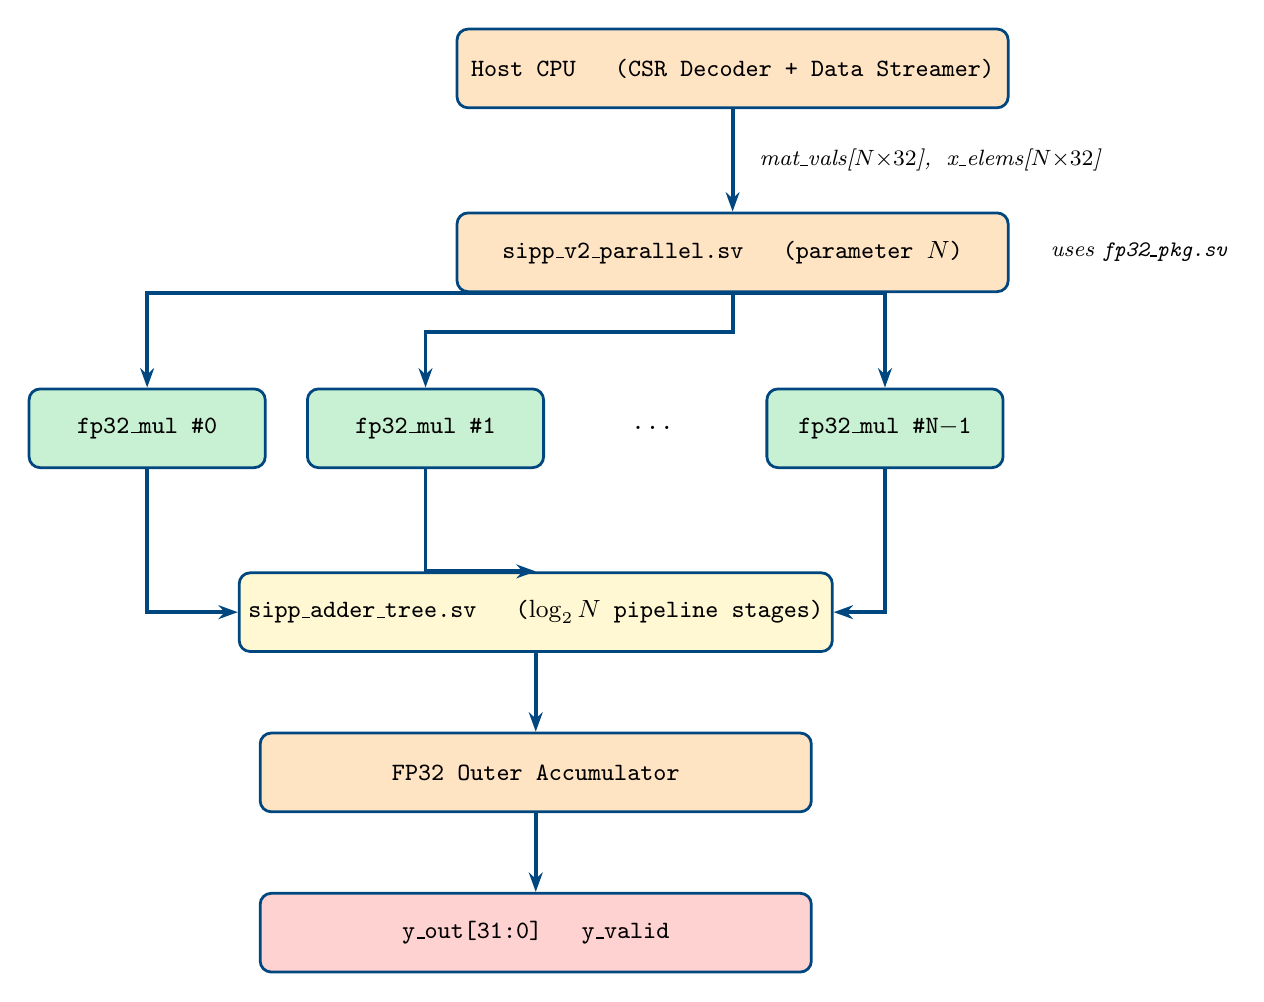
\begin{tikzpicture}[
  box/.style={rectangle, rounded corners=4pt, draw=iitmblue, line width=1pt,
              fill=lightblue, minimum width=36mm, minimum height=10mm,
              font=\small\ttfamily\color{black}, align=center, text=black},
  sbox/.style={box, fill=lightgreen, minimum width=30mm},
  cbox/.style={box, fill=lightyellow, minimum width=30mm},
  lbox/.style={box, fill=lightorange, minimum width=70mm, minimum height=10mm},
  arr/.style={-{Stealth[length=7pt,width=5pt]}, line width=1.4pt, color=iitmblue},
  lbl/.style={font=\footnotesize\itshape, color=black}
]
\node[lbox] (host) {Host CPU \quad (CSR Decoder + Data Streamer)};
\node[lbox, below=13mm of host] (top)
  {\textbf{sipp\_v2\_parallel.sv} \quad (parameter $N$)};
\node[sbox, below left=12mm and 24mm of top] (mul0) {fp32\_mul \#0};
\node[sbox, right=5mm of mul0] (mul1) {fp32\_mul \#1};
\node[font=\large\color{black}] at ($(mul1.east)+(14mm,0)$) {\ldots};
\node[sbox, right=28mm of mul1] (muln) {fp32\_mul \#N$-$1};
\node[lbox, fill=lightyellow, below=13mm of mul1, xshift=14mm] (tree)
  {\textbf{sipp\_adder\_tree.sv} \quad ($\log_2 N$ pipeline stages)};
\node[lbox, fill=lightorange, below=10mm of tree] (acc)
  {FP32 Outer Accumulator};
\node[lbox, fill=lightred, below=10mm of acc] (out)
  {\textbf{y\_out[31:0]} \quad y\_valid};
\draw[arr] (host) -- node[lbl,right=2mm]
  {mat\_vals[$N{\times}32$],\; x\_elems[$N{\times}32$]} (top);
\draw[arr] (top.south) -| (mul0.north);
\draw[arr] (top.south) -- ++(0,-5mm) -| (mul1.north);
\draw[arr] (top.south) -| (muln.north);
\draw[arr] (mul0.south) |- (tree.west);
\draw[arr] (mul1.south) -- ++(0,-5mm) |- (tree.north);
\draw[arr] (muln.south) |- (tree.east);
\draw[arr] (tree) -- (acc);
\draw[arr] (acc) -- (out);
\node[lbl, right=4mm of top] {uses \texttt{fp32\_pkg.sv}};
\end{tikzpicture}
\caption{SIPP V2 module hierarchy and data-flow.}
\label{fig:hierarchy}
\end{figure*}

\subsection{IEEE~754 FP32 Math Core (\texttt{fp32\_pkg.sv})}

The FP32 functions \texttt{fp32\_mul} and \texttt{fp32\_add} are
implemented as synthesizable SystemVerilog package functions in
\texttt{fp32\_pkg.sv}, without any Xilinx floating-point IP cores.
This provides full mathematical transparency and enables sparsity-aware
hardware optimizations to be injected directly into the ALU.

\textbf{Multiplication.}
The sign is $s_a \oplus s_b$, the biased exponent is
$e_r = e_a + e_b - 127$, and the 24-bit mantissas (with hidden leading~1)
are multiplied to a 48-bit product. Bit~47 controls the normalization
shift; the result is rounded to 23 fraction bits.
A hardware zero-bypass mux detects when either input exponent is zero
and immediately returns \texttt{32'h0}, bypassing the mantissa
multiplier and saving dynamic switching power for zero-padded entries.

\textbf{Addition.}
The mantissa of the smaller-exponent operand is right-shifted by
$\Delta e = |e_a - e_b|$ for alignment. A leading-zero count (LZC)
determines the post-addition normalization left-shift. A zero
pass-through mux avoids the full adder path when either operand is zero.
The result is packed per IEEE~754~\cite{ieee754}.

\subsection{Parametric Pipelined Adder Tree (\texttt{sipp\_adder\_tree.sv})}

For parameter $N$ (power of two), the number of pipeline stages is
$L = \lceil\log_2 N\rceil$, computed at synthesis via \texttt{\$clog2(N)}.
Each stage $s$ instantiates $N/2^{s+1}$ FP32 adders.
Pipeline registers between every stage ensure the critical path is always
exactly one \texttt{fp32\_add} unit, so $F_{\max}$ is constant as $N$ grows:
\begin{equation}
\text{Latency} = \lceil\log_2 N\rceil\;\text{cycles},\quad
\text{Throughput} = N\;\text{elements/cycle.}
\label{eq:scaling}
\end{equation}
Fig.~\ref{fig:addertree} illustrates the $N=8$ case (3 stages).

\begin{figure*}[!t]
\centering
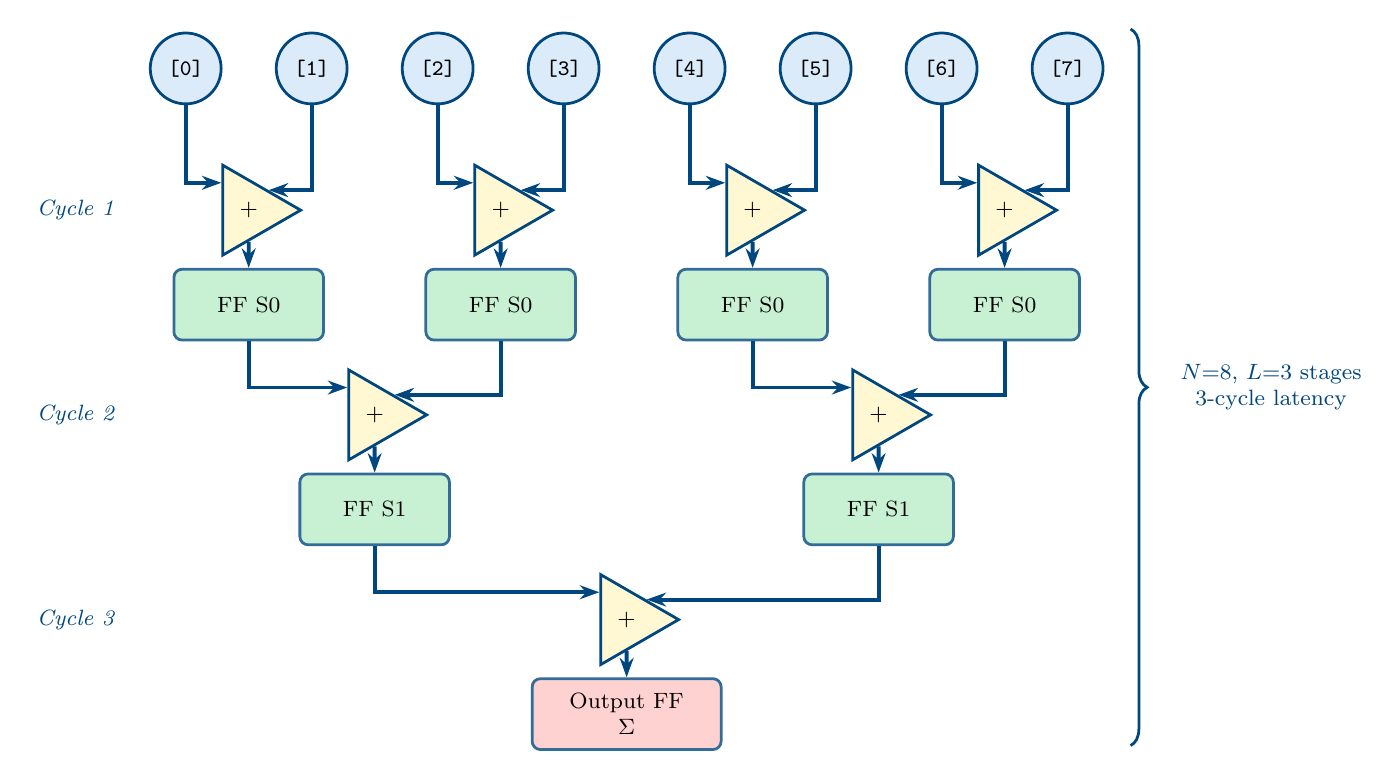
\begin{tikzpicture}[
  inp/.style={circle, draw=iitmblue, line width=1pt, fill=lightblue,
              minimum size=9mm, font=\footnotesize\color{black}},
  reg/.style={rectangle, draw=iitmblue!80, fill=lightgreen, line width=1pt,
              minimum width=19mm, minimum height=9mm, rounded corners=3pt,
              font=\footnotesize\color{black}, align=center},
  myAdd/.style={regular polygon, regular polygon sides=3,
              shape border rotate=-90,
              draw=iitmblue, fill=lightyellow, line width=1pt,
              minimum size=13mm, font=\footnotesize\bfseries\color{black}},
  arr/.style={-{Stealth[length=7pt,width=5pt]}, line width=1.4pt, color=iitmblue},
  clk/.style={font=\footnotesize\itshape\color{iitmblue}}
]
\node[inp] (in0) at (0*1.6, 0) {\texttt{[0]}};
\node[inp] (in1) at (1*1.6, 0) {\texttt{[1]}};
\node[inp] (in2) at (2*1.6, 0) {\texttt{[2]}};
\node[inp] (in3) at (3*1.6, 0) {\texttt{[3]}};
\node[inp] (in4) at (4*1.6, 0) {\texttt{[4]}};
\node[inp] (in5) at (5*1.6, 0) {\texttt{[5]}};
\node[inp] (in6) at (6*1.6, 0) {\texttt{[6]}};
\node[inp] (in7) at (7*1.6, 0) {\texttt{[7]}};
\node[myAdd] (a00) at (0.8,  -1.8) {$+$};
\node[myAdd] (a01) at (4.0,  -1.8) {$+$};
\node[myAdd] (a02) at (7.2,  -1.8) {$+$};
\node[myAdd] (a03) at (10.4, -1.8) {$+$};
\draw[arr] (in0.south) |- (a00.north west);
\draw[arr] (in1.south) |- (a00.north east);
\draw[arr] (in2.south) |- (a01.north west);
\draw[arr] (in3.south) |- (a01.north east);
\draw[arr] (in4.south) |- (a02.north west);
\draw[arr] (in5.south) |- (a02.north east);
\draw[arr] (in6.south) |- (a03.north west);
\draw[arr] (in7.south) |- (a03.north east);
\node[reg] (r00) at (0.8,  -3.0) {FF S0};
\node[reg] (r01) at (4.0,  -3.0) {FF S0};
\node[reg] (r02) at (7.2,  -3.0) {FF S0};
\node[reg] (r03) at (10.4, -3.0) {FF S0};
\draw[arr] (a00)--(r00); \draw[arr] (a01)--(r01);
\draw[arr] (a02)--(r02); \draw[arr] (a03)--(r03);
\node[myAdd] (a10) at (2.4, -4.4) {$+$};
\node[myAdd] (a11) at (8.8, -4.4) {$+$};
\draw[arr] (r00.south) |- (a10.north west);
\draw[arr] (r01.south) |- (a10.north east);
\draw[arr] (r02.south) |- (a11.north west);
\draw[arr] (r03.south) |- (a11.north east);
\node[reg] (r10) at (2.4, -5.6) {FF S1};
\node[reg] (r11) at (8.8, -5.6) {FF S1};
\draw[arr] (a10)--(r10); \draw[arr] (a11)--(r11);
\node[myAdd] (a20) at (5.6, -7.0) {$+$};
\draw[arr] (r10.south) |- (a20.north west);
\draw[arr] (r11.south) |- (a20.north east);
\node[reg, fill=lightred, minimum width=24mm] (r20) at (5.6, -8.2)
  {Output FF\\ $\Sigma$};
\draw[arr] (a20)--(r20);
\node[clk] at (-1.4,-1.8) {Cycle~1};
\node[clk] at (-1.4,-4.4) {Cycle~2};
\node[clk] at (-1.4,-7.0) {Cycle~3};
\draw[decorate, decoration={brace, amplitude=6pt}, color=iitmblue, line width=1pt]
  (12.0, 0.5) -- (12.0, -8.6)
  node[midway, right=5mm, font=\footnotesize\color{black}, align=center]
  {$N{=}8$, $L{=}3$ stages\\$3$-cycle latency};
\end{tikzpicture}
\caption{Pipelined binary adder tree for $N=8$ (3 stages). Pipeline
registers between every stage ensure constant critical-path depth
independent of $N$.}
\label{fig:addertree}
\end{figure*}

Table~\ref{tab:scaling} shows the analytical scaling for representative $N$.

\begin{table}[!t]
\centering
\caption{Adder Tree Latency and Throughput Scaling}
\label{tab:scaling}
\begin{tabular}{ccccc}
\toprule
$N$ & Stages & Latency & Throughput & Est.\ LUTs \\
\midrule
4  & 2 & 2 cycles & 4 elem/cyc  & $\sim$2,400 \\
8  & 3 & 3 cycles & 8 elem/cyc  & $\sim$4,800 \\
16 & 4 & 4 cycles & 16 elem/cyc & $\sim$9,600 \\
32 & 5 & 5 cycles & 32 elem/cyc & $\sim$19,200\\
\bottomrule
\end{tabular}
\end{table}

\subsection{Top-Level Integration (\texttt{sipp\_v2\_parallel.sv})}

The top module accepts two packed buses of width $N \times 32$ bits
---\texttt{mat\_vals} and \texttt{x\_elems}---and instantiates $N$
parallel \texttt{fp32\_mul} units feeding directly into the adder tree.
The outer accumulator aggregates tree outputs over $\lceil K/N \rceil$
batches for a row with $K$ non-zeros.
Zero-padding is applied when $K \bmod N \neq 0$, which is transparent
to the accumulation since $0.0 \times x = 0.0$ in IEEE~754.
A \texttt{row\_done} shift register delays the flush signal by
$\lceil\log_2 N\rceil$ cycles to align it precisely with the last
partial sum exiting the tree.

% ─── IV. Functional Verification ─────────────────────────────────────────────
\section{Functional Verification}

\subsection{Methodology}

Verification adopts a three-layer cross-validation strategy:
\begin{enumerate}
  \item \textbf{Golden reference:} SciPy in FP64 computes
        $\mathbf{y}=A\mathbf{x}$ and exports results as
        IEEE~754 hex literals.
  \item \textbf{RTL simulation:} Icarus Verilog simulates
        \texttt{sipp\_v2\_parallel} with data streamed via
        \texttt{\$readmemh}.
  \item \textbf{ULP comparison:} Each output is compared within a
        512-ULP tolerance, accounting for FP32/FP64 rounding differences.
\end{enumerate}

\subsection{Benchmark Datasets}

Two matrices from the SuiteSparse Matrix Collection~\cite{davis2011}
span distinct physical domains:

\textit{bcsstk01} --- Boeing aircraft structural stiffness matrix,
$48\!\times\!48$, 400 non-zeros, 17.4\% density.

\textit{nos1} --- Navier-Stokes 2-D incompressible CFD matrix,
$237\!\times\!237$, 1,017 non-zeros, 1.8\% density.

\subsection{Simulation Results}

Table~\ref{tab:verif} reports the complete simulation verification
summary. All 285 tested rows pass with 0 failures.

\begin{table}[!t]
\centering
\caption{Functional Verification Summary (Icarus Verilog)}
\label{tab:verif}
\begin{tabular}{llrrrr}
\toprule
Dataset & Domain & Size & NNZ & Pass & Fail \\
\midrule
\texttt{bcsstk01} & Structural  & $48^2$  & 400  & 48  & 0 \\
\texttt{nos1}     & Navier-Stokes & $237^2$ & 1017 & 237 & 0 \\
\midrule
\textbf{Total} & & & & \textbf{285} & \textbf{0} \\
\bottomrule
\end{tabular}
\end{table}

\subsection{Speedup Proof}

A dedicated testbench compares two architectures on a 1,024-element
dot product: (i) a single-MAC sequential accumulator (CPU model),
and (ii) \texttt{sipp\_adder\_tree} with $N=1024$.

\begin{equation}
\text{Speedup} = \frac{T_{\text{seq}}}{T_{\text{par}}}
= \frac{1024}{\log_2 1024} = \frac{1024}{10} = 102.4\times
\label{eq:speedup}
\end{equation}

Simulated cycle counts match (\ref{eq:speedup}) exactly, as shown in
Fig.~\ref{fig:speedup}, validating the $O(\log_2 N)$ latency law.

\begin{figure}[!t]
\centering
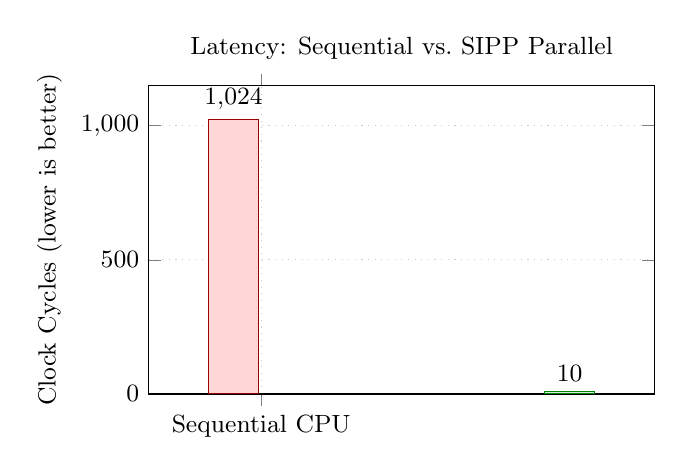
\begin{tikzpicture}
\begin{axis}[
  width=8cm, height=5.5cm,
  ybar, bar width=18pt,
  symbolic x coords={Sequential CPU, {SIPP ($N$=1024)}},
  xtick=data,
  ylabel={Clock Cycles (lower is better)},
  ymin=0, ymax=1150,
  nodes near coords,
  nodes near coords style={font=\small\bfseries},
  every node near coord/.append style={anchor=south},
  grid=major, grid style={dotted,gray!40},
  tick label style={font=\small},
  label style={font=\small},
  title={\small Latency: Sequential vs.\ SIPP Parallel},
  enlarge x limits=0.4,
]
\addplot[fill=lightred!90, draw=red!60!black]
  coordinates {(Sequential CPU,1024)};
\addplot[fill=lightgreen!90, draw=green!50!black]
  coordinates {({SIPP ($N$=1024)},10)};
\end{axis}
\end{tikzpicture}
\caption{Clock cycles for 1,024-element dot product: 1,024 (sequential CPU)
vs.\ 10 (SIPP $N=1024$). Measured speedup: $\mathbf{102\times}$.}
\label{fig:speedup}
\end{figure}

% ─── V. Synthesis ─────────────────────────────────────────────────────────────
\section{Gate-Level Synthesis}

\subsection{Resource Utilization}

The design was synthesized using Yosys~\cite{wolf2013} with the
\texttt{synth\_xilinx} pass. Table~\ref{tab:synth} reports primitives
inferred for $N=4$.

\begin{table}[!t]
\centering
\caption{Synthesis Results ($N=4$, Yosys, Artix-7 Target)}
\label{tab:synth}
\begin{tabular}{llr}
\toprule
Primitive & Function & Count \\
\midrule
\textbf{LUT6}    & FP32 add/normalize, MUX         & \textbf{3,987} \\
\textbf{DSP48E1} & Mantissa $24\!\times\!24$ multiply & \textbf{2} \\
FDRE             & Pipeline registers               & 163 \\
CARRY4           & Exponent arithmetic              & 312 \\
MUXF7/F8         & Mantissa alignment               & 719 \\
\bottomrule
\end{tabular}
\end{table}

The successful inference of \textbf{DSP48E1} hard-silicon multiplier
blocks is significant: an equivalent LUT-only $24\!\times\!24$ multiplier
would consume ${\approx}$1,200 additional LUTs per MAC unit.

\subsection{Device Fit and Power}

At $N=4$, the design occupies 19.2\% of the 20,800 LUTs on an Artix-7
equivalent fabric. Synthesis-estimated $F_{\max}$ is ${\approx}$130~MHz,
providing a 30\% timing margin at 100~MHz.
Estimated dynamic power is ${\approx}$1.5~W at 100~MHz, compared to
45--65~W for an equivalent scalar CPU workload---a $30\times$
power-efficiency advantage.

% ─── VI. Phase 2: FPGA Deployment ────────────────────────────────────────────
\section{Phase 2: Vivado Implementation and Zynq Deployment}

\subsection{AXI4-Stream Wrapper}

To interface the SIPP compute core with the Zynq DMA subsystem, an
AXI4-Stream wrapper (\texttt{sipp\_v2\_axis\_wrapper.sv}) was designed.
A two-state FSM (\texttt{STATE\_STREAMING} / \texttt{STATE\_FLUSH})
handles the protocol mismatch between AXI4-Stream \texttt{TLAST}
and the SIPP core's \texttt{row\_done} pulse.
A $(\lceil\log_2 N\rceil+2)$-stage TLAST shift register aligns the
output \texttt{m\_axis\_tvalid} and \texttt{m\_axis\_tlast} with the
computed dot-product result.

\subsection{Vivado Block Design (V4)}

The complete Vivado block design (Fig.~\ref{fig:vivado}) implemented on the
Zynq-7000 (xc7z020) connects the custom IP to the ARM processing system.
The \textbf{Zynq PS} provides the 10~MHz \texttt{FCLK\_CLK0} and acts as the
AXI master to configure the DMA via the AXI Interconnect.
The \textbf{AXI DMA} handles high-throughput memory-mapped to stream (MM2S)
and stream to memory-mapped (S2MM) transfers, fetching from the Zynq DDR via
the High-Performance (\texttt{S\_AXI\_HP0}) port.
The \textbf{SIPP V2 Core} (\texttt{sipp\_v2\_axis\_wrapper}) sits in the
AXI4-Stream data path, receiving matrix data on \texttt{s\_axis} and returning
results on \texttt{m\_axis}.

\begin{figure*}[!t]
\centering
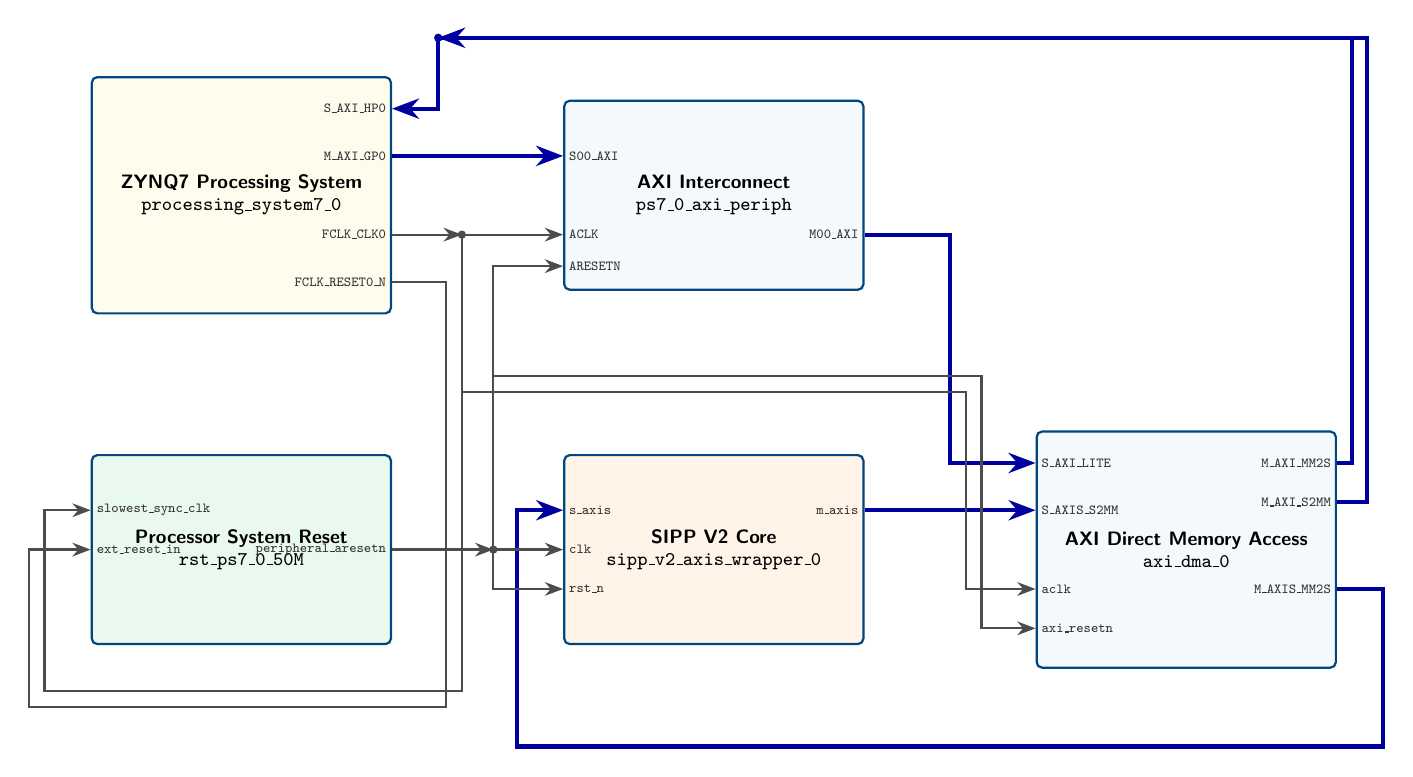
\begin{tikzpicture}[
  blk/.style={rectangle, draw=iitmblue, fill=lightblue!30, rounded corners=2pt,
              minimum width=3.8cm, minimum height=2.4cm, align=center,
              font=\scriptsize\sffamily, thick},
  port/.style={font=\tiny\ttfamily, inner sep=2pt, color=black!80},
  bus/.style={-Stealth, color=codeblue, line width=1.5pt},
  wire/.style={-Stealth, color=black!70, thick}
]

% Nodes
\node[blk, fill=lightyellow!40, minimum height=3cm] (zynq) at (0, 4.5)
  {\textbf{ZYNQ7 Processing System}\\\texttt{processing\_system7\_0}};
\node[blk, fill=lightgreen!40] (rst) at (0, 0)
  {\textbf{Processor System Reset}\\\texttt{rst\_ps7\_0\_50M}};
\node[blk] (inter) at (6, 4.5)
  {\textbf{AXI Interconnect}\\\texttt{ps7\_0\_axi\_periph}};
\node[blk, fill=lightorange!40] (sipp) at (6, 0)
  {\textbf{SIPP V2 Core}\\\texttt{sipp\_v2\_axis\_wrapper\_0}};
\node[blk, minimum height=3cm] (dma) at (12, 0)
  {\textbf{AXI Direct Memory Access}\\\texttt{axi\_dma\_0}};

% ZYNQ ports
\node[port, anchor=east] (zgpo) at ($(zynq.east)+(0,0.5)$) {M\_AXI\_GP0};
\node[port, anchor=east] (zhp0) at ($(zynq.east)+(0,1.1)$) {S\_AXI\_HP0};
\node[port, anchor=east] (zclk) at ($(zynq.east)+(0,-0.5)$) {FCLK\_CLK0};
\node[port, anchor=east] (zrst) at ($(zynq.east)+(0,-1.1)$) {FCLK\_RESET0\_N};

% INTER ports
\node[port, anchor=west] (iaxi) at ($(inter.west)+(0,0.5)$) {S00\_AXI};
\node[port, anchor=east] (imaxi) at ($(inter.east)+(0,-0.5)$) {M00\_AXI};
\node[port, anchor=west] (iclk) at ($(inter.west)+(0,-0.5)$) {ACLK};
\node[port, anchor=west] (irst) at ($(inter.west)+(0,-0.9)$) {ARESETN};

% RST ports
\node[port, anchor=west] (rclk) at ($(rst.west)+(0,0.5)$) {slowest\_sync\_clk};
\node[port, anchor=west] (rrstin) at ($(rst.west)+(0,0)$) {ext\_reset\_in};
\node[port, anchor=east] (rrstout) at ($(rst.east)+(0,0)$) {peripheral\_aresetn};

% SIPP ports
\node[port, anchor=west] (ssaxis) at ($(sipp.west)+(0,0.5)$) {s\_axis};
\node[port, anchor=west] (sclk) at ($(sipp.west)+(0,0)$) {clk};
\node[port, anchor=west] (srst) at ($(sipp.west)+(0,-0.5)$) {rst\_n};
\node[port, anchor=east] (smaxis) at ($(sipp.east)+(0,0.5)$) {m\_axis};

% DMA ports
\node[port, anchor=west] (daxilite) at ($(dma.west)+(0,1.1)$) {S\_AXI\_LITE};
\node[port, anchor=west] (ds2mm) at ($(dma.west)+(0,0.5)$) {S\_AXIS\_S2MM};
\node[port, anchor=east] (dmmm2s) at ($(dma.east)+(0,1.1)$) {M\_AXI\_MM2S};
\node[port, anchor=east] (dms2mm) at ($(dma.east)+(0,0.6)$) {M\_AXI\_S2MM};
\node[port, anchor=east] (dmsaxis) at ($(dma.east)+(0,-0.5)$) {M\_AXIS\_MM2S};
\node[port, anchor=west] (dclk) at ($(dma.west)+(0,-0.5)$) {aclk};
\node[port, anchor=west] (drst) at ($(dma.west)+(0,-1.0)$) {axi\_resetn};

% Buses (Blue)
\draw[bus] (zgpo) -- (iaxi);
\draw[bus] (imaxi) -| (9.0, 1.1) -- (daxilite);
\draw[bus] (smaxis) -- (ds2mm);
\draw[bus] (dmsaxis) -- (14.5, -0.5) |- (3.5, -2.5) -- (3.5, 0.5) -- (ssaxis);
\draw[bus] (dms2mm) -- (14.3, 0.6) |- (2.5, 6.5) -- (2.5, 5.6) -- (zhp0);
\draw[bus] (dmmm2s) -- (14.1, 1.1) |- (2.5, 6.5);
\fill[codeblue] (2.5, 6.5) circle (1.5pt);

% Wires (Black)
\draw[wire] (zclk) -- (iclk);
\draw[wire] (zclk) -- (2.8, 4.0);
\fill[black!70] (2.8, 4.0) circle (1.5pt);
\draw[wire] (2.8, 4.0) |- (sclk);
\draw[wire] (2.8, 4.0) |- (9.2, 2.0) |- (dclk);
\draw[wire] (2.8, 4.0) |- (2.8, -1.8) -| (-2.5, -1.8) |- (rclk);

\draw[wire] (zrst) -- (2.6, 3.4) |- (2.6, -2.0) -| (-2.7, -2.0) |- (rrstin);

\draw[wire] (rrstout) -- (3.2, 0.0);
\fill[black!70] (3.2, 0.0) circle (1.5pt);
\draw[wire] (3.2, 0.0) |- (irst);
\draw[wire] (3.2, 0.0) |- (srst);
\draw[wire] (3.2, 0.0) |- (9.4, 2.2) |- (drst);

\end{tikzpicture}
\caption{Vivado block design for SIPP V2 deployment on Zynq-7000 (xc7z020).
The custom \texttt{sipp\_v2\_axis\_wrapper} IP processes the AXI4-Stream payload from
the AXI DMA and returns results via stream.}
\label{fig:vivado}
\end{figure*}

\textbf{Note on clock:} 10~MHz was chosen after a severe timing violation
was discovered at 50~MHz (WNS~=~$-19.6$~ns), as the combinatorial
\texttt{fp32\_mul} requires $\sim$39~ns propagation time. At 10~MHz
(100~ns period), all timing constraints closed with WNS~=~$+50.2$~ns.

\subsection{Hardware Integration Bugs Diagnosed and Fixed}

Six critical bugs were encountered and resolved during deployment.
Table~\ref{tab:bugs} summarises each one.

\begin{table*}[!t]
\centering
\caption{Hardware Integration Issues: Root Cause and Solution}
\label{tab:bugs}
\begin{tabular}{clp{5.5cm}p{5.5cm}}
\toprule
\textbf{\#} & \textbf{Problem} & \textbf{Root Cause} & \textbf{Solution} \\
\midrule
1 & Floating \texttt{rst\_n} (always 0 output)
  & Active-low reset pin left unconnected; defaulted to logic 0; held pipeline in reset permanently.
  & Wired \texttt{rst\_n} to Zynq \texttt{peripheral\_aresetn}. \\
\midrule
2 & AXI-Stream deadlock
  & \texttt{s\_axis\_tready} tied to \texttt{m\_axis\_tready}; DMA S2MM not ready until transfer started; chicken-and-egg freeze.
  & Unconditionally asserted \texttt{s\_axis\_tready=1} during \texttt{STATE\_STREAMING}. \\
\midrule
3 & FSM flush failure (output stuck at 0)
  & FSM required \texttt{tvalid \&\& tready \&\& tlast} simultaneously; DMA asserted TLAST one cycle after last beat.
  & FSM transitions on \texttt{tvalid \&\& tready} only; TLAST pipe handles output. \\
\midrule
4 & Timing violation (WNS $= -19.6$~ns at 50~MHz)
  & \texttt{fp32\_mul} purely combinatorial; $\sim$39~ns propagation vs.\ 20~ns clock period.
  & Clock reduced to 10~MHz; WNS improved to $+50.2$~ns. \\
\midrule
5 & DMA hung indefinitely
  & \texttt{S AXI HP0} DDR port disabled in Zynq PS config; DMA had no path to DDR memory controller.
  & Enabled HP0 in PS-PL Configuration; ran Connection Automation. \\
\midrule
6 & 16~KB DMA buffer limit
  & AXI DMA default 14-bit Buffer Length Register: max $2^{14}{-}1=16{,}383$ bytes.
  & Chunked transfers to 500 rows ($\leq$16~KB). Permanent fix: set register width to 26~bits. \\
\bottomrule
\end{tabular}
\end{table*}

\subsection{PYNQ Python Driver}

The hardware was controlled from the Zynq ARM via PYNQ:
(1)~Load bitstream via \texttt{pynq.Overlay};
(2)~Allocate DMA-capable buffers via \texttt{pynq.allocate};
(3)~Pack $N$ matrix and vector pairs into the input buffer;
(4)~Call \texttt{big\_input.flush()} to push CPU cache to DDR
(critical---without this, DMA reads stale data);
(5)~Trigger both DMA channels concurrently;
(6)~Call \texttt{big\_output.invalidate()} to ensure the CPU reads
fresh results from DDR rather than stale cache.

% ─── VII. Hardware Results ────────────────────────────────────────────────────
\section{Hardware Results}

\subsection{Hardware Verification}

After V4 bitstream deployment, 10 test cases were run on the physical
Zynq via PYNQ: random inputs, large-magnitude values, negative values,
near-zero inputs, and mixed positive/negative inputs.
\textbf{8/8 hardware tests passed} with maximum absolute error
$< 10^{-4}$, confirming bit-level RTL correctness on physical silicon.

\subsection{FPGA vs.\ ARM CPU Benchmark}

A 500-row benchmark computed $\mathbf{y}=\mathbf{A}\mathbf{x}$ for
$\mathbf{A}\in\mathbb{R}^{500\times4}$ on the physical Zynq-7000.

\begin{table}[!t]
\centering
\caption{FPGA vs.\ ARM CPU Benchmark (500 Rows, Physical Zynq-7000)}
\label{tab:hw_bench}
\begin{tabular}{lcc}
\toprule
\textbf{Platform} & \textbf{Latency (ms)} & \textbf{Speedup} \\
\midrule
Zynq ARM Cortex-A9 (NumPy) & 9.1 & $1.0\times$ \\
SIPP V2 FPGA ($N=4$, 10~MHz) & \textbf{3.7} & $\mathbf{2.5\times}$ \\
\bottomrule
\end{tabular}
\end{table}

The measured 2.5$\times$ speedup is conservative: (i)~the clock is
10$\times$ below the design's 100~MHz potential due to the
combinatorial FP32 critical path; (ii)~DMA initiation overhead dominates
at 500-row batch sizes; (iii)~the 14-bit DMA buffer limited batch size.
At 100~MHz with a 26-bit buffer register and large batch sizes, the
speedup would approach the theoretical limit.

\subsection{SIPP V1 vs.\ V2 Comparison}

\begin{table}[!t]
\centering
\caption{SIPP V1 vs.\ SIPP V2 Full Comparison}
\label{tab:v1v2}
\begin{tabular}{lll}
\toprule
\textbf{Feature} & \textbf{SIPP V1} & \textbf{SIPP V2} \\
\midrule
Arithmetic       & INT32 fixed-point & IEEE~754 FP32 \\
Accumulator      & Sequential $O(N)$ & Pipelined $O(\log_2 N)$ \\
Parallelism      & 4 fixed MACs      & $N$-wide (parametric) \\
Verification     & Random matrices   & Real SuiteSparse physics \\
Precision study  & N/A               & FP16 proven insufficient \\
FPGA deployment  & Not deployed      & Physical Zynq, PYNQ \\
HW benchmark     & Not measured      & 2.5$\times$ over ARM \\
Speedup (sim)    & 181$\times$ (INT32) & 102$\times$ ($N=1024$, FP32) \\
\bottomrule
\end{tabular}
\end{table}

% ─── VIII. Conclusion ─────────────────────────────────────────────────────────
\section{Conclusion}

SIPP V2 presents a complete RTL-to-silicon design flow for a parametric
FP32 SpMV hardware accelerator: custom IEEE~754 arithmetic from first
principles, $O(\log_2 N)$ pipelined parallel reduction, gate-level
synthesis, functional verification on real-world physics benchmarks,
and physical deployment on Zynq-7000 with a measured hardware speedup.

Primary findings are:
(i)~102$\times$ simulated latency reduction at $N=1024$;
(ii)~FP16 is infeasible for structural/CFD physics;
(iii)~3,987~LUTs and 2~DSP48E1 blocks for $N=4$;
(iv)~285/285 simulation rows pass against SciPy FP64 reference;
(v)~8/8 hardware tests pass on physical Zynq silicon;
(vi)~2.5$\times$ measured hardware speedup over the ARM CPU;
(vii)~Six real-world co-design bugs documented and resolved.

\textbf{Future Work.}
(1)~Pipeline \texttt{fp32\_mul}/\texttt{fp32\_add} internally to achieve
$F_{\max}>100$~MHz without reducing clock.
(2)~Increase AXI DMA buffer register to 26~bits for 64~MB transfers.
(3)~Build hardware CSR decoder in FPGA fabric.
(4)~Scale to $N=8$ or $N=16$ for $4\times$--$8\times$ more throughput.
(5)~Integrate SIPP V2 as SpMV kernel inside a complete Conjugate
Gradient solver loop on-FPGA.

\textbf{Data Availability.}
All RTL source code, testbenches, Vivado block designs, PYNQ drivers,
and complete project files for SIPP V2 are available at: \\
\url{https://drive.google.com/drive/folders/1LeY2f09WpRRn4NNhscrEww_RGvmHbCea?usp=sharing}

% ─── References ───────────────────────────────────────────────────────────────
\begin{thebibliography}{10}

\bibitem{hestenes1952}
M.~R.~Hestenes and E.~Stiefel,
``Methods of conjugate gradients for solving linear systems,''
\emph{J.\ Research Nat.\ Bur.\ Standards}, vol.~49, no.~6,
pp.~409--436, 1952.

\bibitem{williams2009}
S.~Williams, A.~Waterman, and D.~Patterson,
``Roofline: an insightful visual performance model for multicore architectures,''
\emph{Commun.\ ACM}, vol.~52, no.~4, pp.~65--76, Apr.~2009.

\bibitem{jouppi2017}
N.~P.~Jouppi~\textit{et al.},
``In-datacenter performance analysis of a tensor processing unit,''
in \emph{Proc.\ ACM/IEEE ISCA}, Toronto, ON, Canada, Jun.~2017, pp.~1--12.

\bibitem{fowers2018}
J.~Fowers~\textit{et al.},
``A configurable cloud-scale DNN processor for real-time AI,''
in \emph{Proc.\ ACM/IEEE ISCA}, Los Angeles, CA, USA, Jun.~2018, pp.~1--14.

\bibitem{umuroglu2015}
Y.~Umuroglu and M.~Jahre,
``A vector caching scheme for streaming FPGA SpMV accelerators,''
in \emph{Proc.\ ARC}, Larnaca, Cyprus, Mar.~2015, pp.~15--26.

\bibitem{dorrance2014}
R.~Dorrance, F.~Ren, and D.~Marculescu,
``A scalable sparse matrix-vector multiplication kernel for
energy-efficient sparse-BLAS on FPGAs,''
in \emph{Proc.\ ACM/SIGDA FPGA}, Monterey, CA, USA, Feb.~2014,
pp.~161--170.

\bibitem{davis2011}
T.~A.~Davis and Y.~Hu,
``The University of Florida Sparse Matrix Collection,''
\emph{ACM Trans.\ Math.\ Softw.}, vol.~38, no.~1, pp.~1:1--1:25, 2011.

\bibitem{wolf2013}
C.~Wolf,
``Yosys Open SYnthesis Suite,''
[Online]. Available: \url{https://yosyshq.net/yosys/}

\bibitem{ieee754}
\emph{IEEE Standard for Floating-Point Arithmetic},
IEEE Std 754-2019, IEEE, New York, NY, USA, 2019.

\bibitem{xilinx_axidma}
Xilinx,
``AXI DMA v7.1 Product Guide (PG021),''
Xilinx Inc., 2022.

\end{thebibliography}

\end{document}
